\documentclass[3p, 11pt]{elsarticle}


%% Use the option review to obtain double line spacing
%% \documentclass[preprint,review,12pt]{elsarticle}

%% Use the options 1p,twocolumn; 3p; 3p,twocolumn; 5p; or 5p,twocolumn
%% for a journal layout:
%% \documentclass[final,1p,times]{elsarticle}
%% \documentclass[final,1p,times,twocolumn]{elsarticle}
%% \documentclass[final,3p,times]{elsarticle}
%% \documentclass[final,3p,times,twocolumn]{elsarticle}
%% \documentclass[final,5p,times]{elsarticle}
%% \documentclass[final,5p,times,twocolumn]{elsarticle}

%% The graphicx package provides the includegraphics command.
\usepackage[utf8]{inputenc}
\usepackage{graphicx}
\usepackage{hyperref}
\usepackage{amssymb}
\usepackage{amsmath}
\usepackage{subcaption}
\journal{EJOR}

\usepackage[mathscr]{eucal}
\newcommand{\R}{\mathbb{R}}
\newcommand{\Co}{\mathbb{Co}}
\newcommand{\D}{\mathscr{D}}
\newcommand{\Pp}{\mathscr{P}}
\newcommand{\Cc}{\mathscr{C}}
\newcommand{\E}{\mathscr{E}}
\newcommand{\F}{\mathscr{F}}
\newcommand{\Ww}{\mathscr{W}}
\newcommand{\Rr}{\mathscr{R}}
\newcommand{\norm}[2][2]{\left\lVert#2\right\rVert_{#1}}
\newcommand{\bigO}{\mathscr{O}}
\newtheorem{thm}{Theorem}
\newtheorem{lem}[thm]{Lemma}
\newdefinition{rmk}{Remark}
\newdefinition{definition}{Definition}
\newproof{pf}{Proof}

\RequirePackage{algorithm, algpseudocode}
\renewcommand{\algorithmicrequire}{\textbf{Input:}}
\renewcommand{\algorithmicensure}{\textbf{Output:}}
\newcommand{\algorithmautorefname}{Algorithm}
\newcommand{\definitionautorefname}{Definition}
\newcommand{\thmautorefname}{Theorem}


\begin{document}
	
	\begin{frontmatter}
		
		%% Title, authors and addresses
		
		\title{Algorithms for Planar Maximum Covering Location by Ellipses Problems\tnoteref{t1}}
		\tnotetext[t1]{This paper is the results of the research
			project funded by CAPES.}
		
		%% use the tnoteref command within \title for footnotes;
		%% use the tnotetext command for the associated footnote;
		%% use the fnref command within \author or \address for footnotes;
		%% use the fntext command for the associated footnote;
		%% use the corref command within \author for corresponding author footnotes;
		%% use the cortext command for the associated footnote;
		%% use the ead command for the email address,
		%% and the form \ead[url] for the home page:
		%%
		%% \title{Title\tnoteref{label1}}
		%% \tnotetext[label1]{}
		%% \author{Name\corref{cor1}\fnref{label2}}
		%% \ead{email address}
		%% \ead[url]{home page}
		%% \fntext[label2]{}
		%% \cortext[cor1]{}
		%% \address{Address\fnref{label3}}
		%% \fntext[label3]{}
		
		
		%% use optional labels to link authors explicitly to addresses:
		%% \author[label1,label2]{<author name>}
		%% \address[label1]{<address>}
		%% \address[label2]{<address>}
		
		\author[1]{Danilo Tedeschi}
		\ead{danilo.tedeschi@usp.br}

		
		\author[2]{Marina Andretta}
		\ead{andretta@gmail.com}
					
		%\address{Department of Applied Mathematics and Statistics, Institute of Mathematical and Computer Sciences, University of São Paulo, Avenida Trabalhador São-carlense, 400, Centro, 13566-590, São Carlos, SP, Brazil.}
		%\author{John Smith}
		
		%address{California, United States}
		
		\begin{abstract}
			%% Text of abstract
			Planar Maximum Covering Location by Ellipses is an optimization problem where one wants to place fixed shape ellipses on the plane to cover demand points
			maximizing a function depending on the value of covered points.
			We propose new exact algorithms for two versions of this problem, one where the ellipses have to be parallel to the coordinate axis, and another where they can be freely rotated. 
			Besides finding optimal solutions for previously published instances, including the ones where no optimal solution was known, both algorithms proposed by us were able to obtain optimal solutions for some new larger instances having with up to seven hundred demand points and five ellipses.
		\end{abstract}
		
		\begin{keyword}
			Optimization \sep Covering \sep Combinatorial Optimization
			%% keywords here, in the form: keyword \sep keyword
			
			%% MSC codes here, in the form: \MSC code \sep code
			%% or \MSC[2008] code \sep code (2000 is the default)
			
		\end{keyword}
		
	\end{frontmatter}
	
	%%
	%% Start line numbering here if you want
	%%
	%\linenumbers
	
	%% main text
	\section{Introduction}
	
	The Planar Maximum Covering Location Problem (PMCLP) was first introduced in \cite{church:1984}, and can be seen as a category of problems where the coverage of a demand set, a collection of subsets of $\R^2$, is to be maximized by determining the location of facilities in $\R^2$, with coverage being determined by a distance function.
	In \cite{church:1984}, methods for Euclidean and Rectilinear distances versions of the problem were proposed.
	In \cite{drezner, chazelle:1986}, exact algorithms for the Euclidean PMCLP with only one facility are proposed; and in \cite{cabello:2006} an approximation algorithm is proposed for the version with multiple unit disks as facilities.
	A property of the Euclidean PMCLP, which is utilized in the algorithms developed in \cite{drezner, chazelle:1986, cabello:2006}, and in the method proposed in \cite{church:1984}, is that there is an optimal solution which every facility is located in the demand points, or in the intersection of two circles centered at two demand points; we will prove a similar property for ellipses in our work.
	
	It is fair to say that PMCLP with elliptical coverage has not been vastly studied as only two articles have been found on it. In \cite{canbolat}, a mixed-integer non-linear programming method was proposed as a first approach to the problem. For some instances, the method took too long and did not find an optimal solution. Because of that, a heuristic method was developed using a technique called Simulated Annealing, which was able to obtain solutions for the instances proposed in that study.
	The problem was further explored in \cite{andreta}, which introduced the version where the ellipses can be freely rotated, to which an exact and a heuristic method was proposed, and developed a new method for the axis-parallel version of the problem, which was able to obtain optimal solutions for instances that the method proposed by \cite{canbolat} could not.
	The exact method for the version with rotation could not obtain optimal solutions within a predefined time limit for several instances, the heuristic method though returned solutions for every instance, and impressively enough, obtained optimal solutions for every verifiable instance.
	
	We study two versions of PMCLP with elliptical coverage facilities in this work. For both of them, each ellipse is defined to have a fixed shape and an undefined location, which is part of the solution.
	In the first version, introduced in \cite{canbolat}, all the ellipses are restricted to be axis-parallel, while in the second version, introduced in \cite{andreta}, this constraint is dropped, and all the ellipses can be freely rotated.
	The first version will be referred to as Planar Maximum Covering Location by Ellipses Problem (MCE) and the second one as  Planar Maximum Covering Location by Ellipses with Rotation Problem (MCER).
	
	\section{Problem Definition}
	
	An instance of MCE and MCER is given by $n$ demand points $\Pp=\{p_1, \dots, p_n\}$, $p_j\in\R^2$; $n$ weights $\Ww=\{w_1, \dots, w_n\}$, with $w_j\in\R$, $w_j>0$ being the weight of the $j$-th point; and $m$ shape parameters $\Rr=\{(a_1, b_1), \dots, (a_m, b_m)\}$, with $(a_j, b_j)$ being the semi-major and semi-minor of the $j$-th ellipse, with $a_j > b_j$. We define a list of functions $\E=\{E_1, \dots, E_m\}$ representing the coverage area of each facility. For MCE $E_j\colon\R^2\to\R^2$ is defined as
	\begin{equation}
	E_j(q) = \{p \in \R^2 \colon (p_x-q_x)^2/a_j^2 + (p_y-q_y)^2/b_j^2 \le 1\}.
	\end{equation}
	For MCER, we define $E_j \colon \R^2 \to \R^2 \times [0, \pi)$ as
	\begin{equation}
		E_j(q, \theta) = \left\{p \in \R^2 \colon 
		\left|\left|
		\left(
		\begin{array}{rr}
		\cos{\theta}/a_j & \sin{\theta}/a_j\\
		\sin{\theta}/b_j & -\cos{\theta}/b_j
		\end{array}
		\right)
		\left(
		\begin{array}{c}
		p_x-q_x\\
		p_y-q_y
		\end{array}
		\right)
		\right|\right|_2
		\le 1
		\right\}.
	\end{equation}
	
Let $w : A \subset \Pp \to \R$ be a function which takes a subset of the demand set and returns the sum of the weights of the points in $A$. Then, we define MCE as the optimization problem 
\begin{equation}
\max_{q_1, \dots, q_m} \sum_{j=1}^m w(\Pp \cap E_j(q_j)),
\end{equation}
and similarly MCER as
\begin{equation}
\max_{(q_1, \theta_1), \dots, (q_m, \theta_m)} \sum_{j=1}^m w(\Pp \cap E_j(q_j, \theta_j)).
\end{equation}

To make the notation more clear, we denote an instance of MCE or MCER as the tuple $(\Pp, \Ww, \Rr)$, and a solution of MCE as $Q:=(q_1, \dots, q_m)$, and a solution of MCER as $Q:=((q_1, \theta_1); \dots; (q_m, \theta_m))$. We also use $\partial$ as the boundary operator, for example, $\partial E_1(q_1)$ denotes an ellipse with shape parameters $(a_1, b_1)$ centered at $q_1$ given an instance of MCE.

\section{An algorithm for MCE}

We will develop a method which is similar to the one developed in \cite{drezner} for only one euclidean disk, and the exact algorithm developed for multiple Euclidean disks in \cite{cabello:2006}. 
We first describe a Candidate List set (CLS) for each facility, which is finite set of possible locations for each ellipse, which we use to converting MCE into a discrete optimization problem. We, then prove that using the possible solutions obtained from the combination of every ellipse's CLS an optimal solution can be obtained.

%\subsection{An equivalent problem}

Let $(\Pp, \Ww, \Rr)$ be an instance of MCE, then for each $j=1\dots m$, consider $n$ ellipses with shape parameters $(a_j, b_j)$ centered at each one of the points in $\Pp$. If we have $q_j\in\R^2$ in a subset of the coverage areas of those ellipses, then $q_j$ is a solution of MCE covering the centers of those ellipses. In other words, if $q_j \in \R^2$, and $X \subset \{1, \dots, n\}$, $X \neq \emptyset$, such that $q_j \in \cap_{i\in X}E_j(p_i)$, then $\Pp \cap E_j(q_j) = \{p_i \colon i \in X\}$.
From that observation, we can constrain each $q_j$ to be in $\cap_{i\in X} E_j(p_i)$, for some $X \subset \{1, \dots,n\}$, $X \neq \emptyset$.

In \cite{bi}, an algorithm is proposed for the problem of determining the intersection of disks of fixed radii from a strictly convex normed plane. 
We say that $(\R^2, ||\cdot||)$ is a strictly convex normed plane if the unit disk given by the norm $||\cdot||$ is strictly convex. Note that for any ellipse, there is a strictly convex normed plane whose unit circle is that ellipse.
For that reason, we state some results from \cite{bi} here, which we use on the development of an algorithm for MCE.


Let $(\R^2, ||\cdot||)$ be a strictly convex normed plane, and $\D=\{D_1, \dots, D_n\}$ be a set of $n$ unit disks in that space centered at different points, with the condition that  $\cap_{i=1}^n D_i \neq \emptyset$. In \cite{bi}, an algorithm was developed to construct this intersection in $\bigO(n\lg{n})$, some of its preliminary results are:
\begin{itemize}
	\item $\partial \cap_{i=1}^n D_i$ is formed by arcs of $\partial D_1, \dots, \partial D_n$.
	\item The vertices of $\partial \cap_{i=1}^n D_i$ is contained in the set of pairwise-intersection of the circles $\partial D_1, \dots, \partial D_n$.
	\item $|\partial D_i \cap \partial D_j| \le 2$.
\end{itemize}

Based on those, we introduce the next definition for the $k$-th ellipse's CLS, which we refer to as $S_k$.

\begin{definition}\label{def:cls_mce}
	Given an instance of MCE, for any $k \in \{1, \dots, m\}$, we define the CLS for the $k$-th ellipse as
	\begin{equation}
	S_k = \bigcup_{1 \le i < j \le n} \partial E_k(p_i) \cap \partial E_k(p_j) \bigcup \Pp.
	\end{equation}
\end{definition}

The set of solutions $S_k$, can be computed in $\bigO(n^2)$ as determining the intersections between two axis-parallel ellipses can be done analytically. 

\begin{lem}
	Given an instance of MCE, and $S_1, \dots, S_m$ as defined by \autoref{def:cls_mce}, then the set $\Omega = \{(q_1, \dots, q_m) \colon \textnormal{ for all }q_k \in S_k \}$ contains an optimal solution of MCE and $|\Omega| \le n^{2m}$. 
\end{lem}
\begin{pf}
	Let $Q^*$ be an optimal solution of MCE for the given instance. Then, we are going to prove that there exists $Q' \in \Omega$, which is also optimal.
	
	For each $k=1, \dots, m$, let $X_k = \{p_i \in \Pp\colon p_i \in E_k(q_k^*)\}$.
	
	If $|X_k| = 0$, then any $q_k \in S_k$ makes $X_k \subset \Pp \cap E_k(q_k)$.
	
	if $|X_k| = 1$, then there is at least one element in $S_k$ that makes $X_k \subset \Pp \cap E_k(q_k)$.
	
	if $|X_k| > 1$, then let $Y_k = \cap_{p \in X_k}E_k(p)$, by the results of \cite{bi}, we have that the boundary of $Y_k$ has vertices in the pairwise intersections of $\{\partial E_k(p) \colon p \in X_k\}$. Therefore, at least one vertex of $Y_k$ is in $S_k$, and any of those vertices produce a solution that covers at least the same points covered by $Q^*$.
	
	Lastly, we have that $|S_k| \le 2\binom{n}{2} + n = n(n+1)/2 \le n^2$ hence $|\Omega| \le n^{2m}$.
\end{pf}

With all this in hand, we can go ahead and define an algorithm for MCE.

\begin{algorithm}
	\caption{Algorithm for MCE}\label{algoritmo:mce}
	
	\begin{algorithmic}[1]
		\Require{A set of points $\Pp=\{p_1,\dots,p_n\}$, a list of weights $\Ww=\{w_1, \dots, w_n\}$, and a list of shape parameters $\Rr=\{(a_1, b_1), \dots, (a_m, b_m)\}$.}
		
		\Ensure{An optimal solution for MCE.}
		
		\item[]
		\Procedure{$MCE$}{$\Pp, \Ww, \Rr$}
		\State \Return $MCE_{bt}(\Pp, \Ww, \Rr, 1)$
		\EndProcedure
		\State
		\Procedure{$MCE_{bt}$}{$Z, \Ww, \Rr, j$}
		\If{$j = m+1$}
		\State \Return $0$
		\EndIf
		
		\State $(q_j^*, \dots, q_m^*) \gets (0, \dots, 0)$
		\State Let $S_j$ be the CLS for the $j$-th ellipse as defined by \autoref{def:cls_mce}.
		%\State $S_j \gets \textnormal{CLS-MCE}(Z, a_j, b_j)$
		\For{$q_j \in S_j$}
		\State $Cov \gets \Pp \cap E_j(q_j)$
		\State $(q_{j+1}, \dots, q_m) \gets MCE_{bt}(Z \setminus Cov, \Ww, \Rr, j+1)\}$
		
		\If{$w(\cup_{k=j}^m Z \cap E_k(q_k)) >  w(\cup_{k=j}^m Z \cap E_k(q_k^*))$}
		\State $(q_j^*, \dots, q_m^*) \gets(q_j, \dots, q_m)$
		\EndIf
		\EndFor
		
		\State \Return $(q_j^*, \dots, q_m^*)$
		\EndProcedure
	\end{algorithmic}
\end{algorithm}

\autoref{algoritmo:mce} can be proved to have a runtime complexity of $\bigO(mn^{2m+1})$.

\section{Determining every location of an ellipse given its shape and three points}
	
The problem of finding every center and angle of rotation of a fixed shape ellipse which makes it have three points on its border is presented in this section. Even though its simple statement--it is short and uses only basic mathematical concepts--we were not able to find any work on it, or even on related problems. 
As a result, starting from scratch, we ended up trying a handful of approaches with most of them failing on the way. We try to give a review of some of those, and also make a case for the method we propose in terms of velocity of convergence and quality of the solutions that it finds.

We refer to this problem as \sigla{E3PNT}{Ellipse by Three points}, and an instance of it is given by three points $u, v, w \in \R^2$ and $E$, an ellipse with shape parameters $(a, b) \in \R^2_{>0}$, with $a > b$. A solution of E3PNT is a pair $(q, \theta) \in \R^2\times[0, \pi]$, such that $\{u, v, w\} \subset \tilde{E}(q, \theta)$. In other words, the goal is to develop a method to find every solution of E3PNT. 


\section{Transforming the problem}

To make it simpler, let us translate the system, so the point $u$ is at $(0,0)$. Then, we assume that the ellipse is actually axis-parallel and the points are the ones rotating. When an angle is found such that the three points lie on the border of the axis-parallel ellipse, a linear transformation can be applied to compress the x-axis by $\frac{b}{a}$, transforming the ellipse into a circle of radius $b$. This transformation can be seen on \autoref{fig:circumscribed-circle} where a solution of the E3PNT is transformed into a solution of the problem of finding a circumscribed circle of a triangle. 
This process can be parametrized by the angle of rotation of the points, as described by \autoref{eq:trpnts}, and because of the invertibility of linear transformations solutions for E3PNT can be obtained by reversing the transformations.

\begin{figure}
	\centering
	\caption{Transforming an ellipse into a circle. T1, T2, and T3 represent the steps of the transformation.}
	\includegraphics{tex/figures/scripts/circumscribed-circle}
	\fautor
	\label{fig:circumscribed-circle}
\end{figure}
\begin{equation}\label{eq:trpnts}
\varphi(p, \theta)=\left[\begin{array}{cc}
\frac{b}{a}&0\\
0&1
\end{array}\right]
\left[\begin{array}{cc}
\cos{\theta}&\sin{\theta}\\
-\sin{\theta}&\cos{\theta}
\end{array}\right]\left[\begin{array}{c}
p_x\\
p_y
\end{array}\right].
\end{equation}

Then, the problem to be solved is finding a circumscribed circle of the triangle formed by the points $(0, 0), \varphi(v, \theta)$ and $\varphi(w, \theta)$, such that the circle has radius $b$. As, for three non-colinear fixed points, there is always an unique circumscribed circle for the triangle formed by those three points, the only variable to be determined ends up being the angle of rotation $\theta$.

Let $A(\theta)$ be the area of the triangle formed by the points $(0, 0), \varphi(v, \theta)$ and $\varphi(w, \theta)$--note that the transformation does not preserve distance or area. Then, the radius $R$ of the circumscribed circle is given by \autoref{eq:circumscribed_circle} \cite[p.~189]{johnson1960}.

\begin{equation}\label{eq:circumscribed_circle}
R = \dfrac{\norm{\varphi(v, \theta)}\norm{\varphi(w, \theta)}\norm{\varphi(v, \theta)-\varphi(w, \theta)}   }{4A(\theta)}.
\end{equation}

Imposing the radius to be equal $b$ and squaring to eliminate the square roots present in the Euclidean distance, a function $\xi : [0, \pi) \mapsto \mathbb{R}_{>0}$ is defined by \autoref{eq:circumscribed_circle_b} in such a way that its zeros determine solutions to the E3PNT's instance. Two questions about $\xi(\theta)$ that arise are: is its set of roots finite? And, can they be found analytically?

\begin{equation}\label{eq:circumscribed_circle_b}
\xi(\theta) = 16b^2A(\theta)^2 - \norm{\varphi(v, \theta)}^2\norm{\varphi(w, \theta)}^2\norm{\varphi(v, \theta)-\varphi(w, \theta)}^2.
\end{equation}

\subsection{The number of solutions is limited}

The method developed on \autoref{chapter:ellipses_n} iterates over every solution of E3PNT for every triplet of points, this is only possible if the size of this set of solutions is limited. Also, if this was not true, it would be very difficult to describe a method to get every solution which could be infinite.

It turns out that $\xi$ can be written as a real trigonometric polynomial of degree $6$ in the format given by \autoref{eq:trig_poly_2}, which implies that it can have up to $12$ distinct roots.
 To show that, just note that it is possible to write $\norm{\varphi(v, \theta)}^2$ and $A(\theta)^2$ in that form, as it can be seen on \autoref{eq:dd} and \autoref{eq:dd2}. It is also possible to see that the term of higher the degree of $\xi$ is the multiplication of the three squared distances. As $\norm{\varphi(v, \theta)}^2$ has degree $2$, the degree of $\xi$ is $6$.
\begin{align}\label{eq:dd}
	\norm{\varphi(v, \theta)}^2 = (v_x\frac{b}{a}\cos\theta + v_y\frac{b}{a}\sin\theta)^2 + (v_y\cos\theta - v_x\sin\theta)^2\\
	\label{eq:dd2} A(\theta)^2=\dfrac{1}{4}\det\left(
	\begin{array}{cc}
		v_x\frac{b}{a}\cos\theta + v_y\frac{b}{a}\sin\theta&v_y\cos\theta - v_x\sin\theta\\
		w_x\frac{b}{a}\cos\theta + w_y\frac{b}{a}\sin\theta&w_y\cos\theta - w_x\sin\theta
	\end{array}\right)^2
\end{align}

Because ellipses are symmetrical with respect to their major-axis, and any rotation in the interval $[0, \pi)$ is identical to a rotation in $[\pi, 2\pi)$, the number of different solutions is cut in half.
Therefore, the number of angles of rotation and centers that an ellipse of fixed shape can be placed, so it has three fixed points on its border is limited to $6$.

\section{An attempt using the conic general equation}

The idea of this approach was to use the six-parameter conic equation to represent an ellipse. This equation is given by \autoref{eq:gen_ellipse}.

\begin{equation}\label{eq:gen_ellipse}
Ax^2+Bxy+Cy^2+Dy+Ex+F=0.
\end{equation}
This equation actually represents any conic, for it to be an ellipse the condition $B^2 -4AC < 0$ must be satisfied.

Setting the first point to be the origin, we get $F=0$, using the other two points, it is possible to write $D$ and $E$ in terms of $A, B, C$. As any multiple of \autoref{eq:gen_ellipse} represents the same conic, we can set $B$ to be equal $1$. Then, we end up with two variables, $A$ and $C$, and still need to impose that the final equation represents an ellipse and its major-axis and minor-axis have the predefined value. Let $\Delta=4AC-B^2=4AC-1$, \autoref{eq:gen_ellipse_a} and \autoref{eq:gen_ellipse_b} for both major-axis and minor-axis respectively, assuming $F=0$.

\begin{align}\label{eq:gen_ellipse_a}
a^2 = \dfrac{2\dfrac{AE^2 -BDE +CD^2}{\Delta}}{A + C - \sqrt{1 + (A-C)^2}}\\
\label{eq:gen_ellipse_b}b^2 = \frac{2\dfrac{AE^2 -BDE +CD^2}{\Delta}}{A + C + \sqrt{1 + (A-C)^2}}
\end{align}

These two equations define two curves in $\R^2$ with $A$ and $C$ being the chosen variables. The solutions lie in the set of intersection of these curves. Finding this set was judged to be non-trivial and probably could be approximated numerically, however, we decided not to further pursue this approach.

Another idea which has been explored was working with the ratio $\frac{a^2}{b^2}$ which becomes an expression that allows $A$ to be written as a function of $C$. This function appeared, at first we thought, to be monotonic, we tried to develop a method based on that, however, cases where the function does not behave as nicely were found. It is likely that developing a method to approximate solutions working with this function is possible, but we decided not to continue on this track.


\section{An approximation method}

One of the most useful techniques when dealing with complicated functions is approximation. They appear in various methods whenever a derivative or integral needs to be calculated or for example, in our case, when the roots of a function need to be determined. In general, one has a function $f$ that is part of a family of functions $\mathcal{A}$ and wants to select a simpler function $f^*$ from a set of functions $\mathcal{A^*}$, such that $f^*$ is close enough to $f$ \cite[p.~3]{powell}. For this problem, the approximation of $\xi(\theta)$ on the interval $[0, \pi)$ is considered. The approximation set of functions is going to be the set of $n$-degree Chebyshev polynomials which the roots can be found through determining the eigenvalues of a $n$ by $n$ matrix.


\subsection{Chebyshev interpolation}

Chebyshev polynomials are widely used in Numerical Analysis in areas like numerical integration, polynomial approximation, and ordinary and partial differential equations.
They are also very useful in practice and are present in extension libraries in Python and MATLAB.

Because of the scope of this work, only a brief introduction of Chebyshev polynomials of the first kind and its usage in polynomial interpolation is given. For a more thorough work on the subject, please check the book by \citeonline{chebbook}.

We refer to $T_n : [-1, 1] \mapsto [-1, 1]$ as the $n$-degree Chebyshev polynomial of the first kind, and it is defined as follows:

\begin{equation}
T_n(x) = \cos({n\arccos x})
\end{equation}

It is important to mention that this definition can be extended to the whole real line. Using some trigonometric identities, $T_n$ can also be expressed as a recurrence relation:

\begin{equation}
T_n(x) = 2xT_{n-1}(x) - T_{n-2}(x).
\end{equation}

An important property worth bringing up is that Chebyshev polynomials are orthogonal and form a basis for the polynomial space. This implies that any $p_n$ of degree up to $n$ can be expressed as a truncated Chebyshev series:

\begin{equation}\label{eq:chebseries}
p_n(x) = \sum_{j=0}^{n} a_j T_j(x).
\end{equation}

One of the greatest qualities of Chebyshev polynomials is its numerical stability. \citeonline{gautschi:1979} showed that the matrix that maps polynomials onto its coefficients written in the power form\footnote{A polynomial is in the power form or the monomial form if it can be written as $\sum_{j=0}^{n}a_jx^j$} has a condition number that grows exponentially with $n$. On the other hand, the matrix that converts polynomials to the Chebyshev basis as \autoref{eq:chebseries}, has a linear condition number bounded by $\sqrt{2}n$.

Polynomial interpolation is a form of approximating a function by a polynomial of degree $n$ that passes through $n+1$ chosen points. In fact, this polynomial is unique and it is determined by Lagrange's formula:

\begin{equation}\label{eq:lagrange}
f_n(x) = \sum_{j=0}^{n} f(x_j)\dfrac{\prod_{k \neq j}^{n+1} (x-x_k)}{\prod_{k \neq j}^{n+1} (x_j-x_k)},
\end{equation} 
with $f$ being the function to be approximated, and $f_n$ the unique $n$-degree polynomial that passes through $\{(x_j, f(x_j)): j=0, 1, \dots n\}$. Because of the uniqueness of interpolant polynomials, there is a direct link between the quality of an approximation and the points chosen to interpolate. As a matter of fact, depending on the points one chooses, even increasing the degree of the interpolation makes the approximation worsen. This is known as Runge's phenomenon and an example can be seen in \citeonline[p.~37]{powell} where uniformly spaced points are chosen to interpolate the function $f(x) = (1+x^2)^{-1}$ on the interval $[-5, 5]$. 

That is where Chebyshev interpolation comes in. Instead of choosing $n+1$ arbitrary points, the $n+1$ roots of $T_{n+1}$, which are also known as Chebyshev Nodes, are chosen as the interpolation points:
\begin{equation}
x_j = \cos{\left(\dfrac{\pi(k-\frac{1}{2})}{n+1}\right)},
\end{equation}
for $j=1, \dots, n+1$. This particular choice defeats Runge's phenomenon and provides a convergent approximation. 

Note that, if the domain of the function to be interpolated is defined on a range other than $[-1, 1]$, let us say $[a, b]$, then a transformation can be done to map it to the Chebyshev Nodes' domain:
\begin{equation}
\hat{x_j} = \frac{a+b}{2} + \frac{b-a}{2}x_j.
\end{equation}

Then, the Chebyshev interpolation of a function $f: [a, b] \mapsto \R$ can be determined using Lagrange's formula and the points $\hat{x}_1, \dots, \hat{x}_n$. 
As it was mentioned, finding the roots of a polynomial written in the monomial form can be done by determining the eigenvalues of a so-called Frobenius companion matrix. For small $n$ this works fine, however, converting the polynomial obtained by \autoref{eq:lagrange} to the power form, as $n$ grows, becomes a very ill-conditioned problem. 
An alternative method can be found in \citeonline{boyd:2013} where the Chebyshev interpolation is calculated directly as a truncated Chebyshev series, as in \autoref{eq:chebseries}, in $\bigO(n^2)$. Also, given a polynomial written in the Chebyshev basis, a $n\times n$ matrix can be constructed, such that its eigenvalues are the roots of that polynomial. \citeonline{boyd:2013} refers to this matrix as the Chebyshev-Frobenius companion matrix.

Therefore, the whole process of interpolating and finding the roots can be done using only Chebyshev polynomials, which have great numerical stability. Also, Chebyshev-Frobenius matrices have the same property as companion matrices which allows their eigenvalues to be found by a QR decomposition. Summing the two steps, a $\bigO(n^2)$ algorithm can be achieved.

The last question that needs to be addressed is how close the roots of the Chebyshev interpolant $f_n$ are to the roots of $\xi$?

Even though $\xi$ is complicated enough, in a sense that finding its roots directly is no trivial task, it is a very well-behaved function: it is analytic and  has infinitely many continuous and integrable derivatives. This satisfy all the requirements of the result in \citeonline[p.~28]{gottlieb} which says that if a function has $m$ continuous and integrable derivatives on a closed interval, then its absolute difference between the Chebyshev truncate series is $\bigO(n^{-m})$. Also, in \citeonline{battles:2004} a theorem is presented stating that if a function is analytic on a neighborhood of $[-1, 1]$, then the convergence is $\bigO(C^n)$, for some $C<1$.

To choose the degree of the interpolation we use the last coefficient rule-of-thumb introduced by \citeonline[p.~50]{boyd:2001}. There is no guarantee that this method will choose $n$, such that $f_n$ is close enough to $\xi$ everywhere on $[0, \pi)$, nonetheless, in practice, it is taken to be a good estimate for the error $r_n$:
\begin{equation}
r_n = \max_{0 \le \theta \le \pi} |f_n(\theta) - \xi(\theta)|.
\end{equation}


\section{Converting $\xi$ into a polynomial}

On \autoref{chapter:definitions} a brief introduction is given on how to get the roots of a polynomial. For that reason, we discuss two ways of converting $\xi$ into a polynomial in this section. Symbolic computing was used to compute the polynomials, in practice an external Python library called SymPy was utilized (see \citeonline{sympy} for more details).

The first attempt was using the identity $x = \tan{\frac{\theta}{2}}$ from which it is possible to construct a $12$-degree polynomial. At first,  the root-finding algorithm described on \autoref{chapter:definitions} seemed to work fine and return every solution of E3PNT, however, we later found out that for some instances, priorly known roots were not being found. The cause was not for sure identified, but a good guess would be that for angles which are greater than $\frac{\pi}{4}$, $x$ starts growing too rapidly which could lead to numerical instability.

The second approach is based on a idea published on \citeonline{boyd:2006} which uses the identities on \autoref{eq:complex_trig} to convert real trigonometric polynomials into univariate complex polynomials in order to obtain its roots using the companion matrix scheme.
Also, in \citeonline{weidner} it is said that computing the roots of a real trigonometric polynomial through this transformation does not yield loss of accuracy.

\begin{align}\label{eq:complex_trig}
\cos{\theta} = \dfrac{e^{i\theta} + e^{-i\theta}}{2}\\
\sin{\theta} = \dfrac{e^{i\theta} - e^{-i\theta}}{2i}.
\end{align}

It is possible to show that with that substitution and changing the variable to $z=e^{i\theta}$, we obtain the following function $g : \mathbb{S} \mapsto \mathbb{C}$, with $\mathbb{S}$ being the unit circle ($\mathbb{S} = \{z \in \mathbb{C} : |z|=1\}$):

\begin{equation}
g(z)=\sum_{k=0}^{12} c_k z^{k-6},
\end{equation}
for some $c_0, \dots, c_{12} \in \mathbb{C}$. Even though $g$ is not a polynomial, it is easy to obtain one from it. Firstly, the negative exponentials need to be shifted, this can be done by just multiplying $g$ by $z^6$. Secondly, the domain cannot be restricted to the unit circle, so we define $h : \mathbb{C} \mapsto \mathbb{C}$ as:
\begin{equation}
h(z) = z^6 g(z) = \sum_{k=0}^{12} c_k z^k.
\end{equation}

Then, by its definition is possible to see that every root of $g$ is also a root of $h$. Conversely, every root $\hat{z}$ of $h$ which is in $\mathbb{S}$--or $|\hat{z}|=1$--is also a root of $g$. Naturally, the angle of a root $\hat{z}$ of $g$ is a root of $\xi$ by Euler's Formula.

It is possible to make another reduction to obtain a degree-$6$ polynomial from $h$ whose roots form a superset of the roots of $g$. As it has been mentioned on this chapter, an ellipse is symmetric with respect to its own axis. This means $\theta$ and $\pi + \theta$ are equivalent angles of rotation for any ellipse, thus $\xi(\theta) = \xi(\pi + \theta)$\footnote{$\xi$ is only defined over $[0, \pi)$, so this equality is not actually valid.}. 
On \autoref{chapter:definitions}, it was stated that the angle of $z$ and $-z$ has the same symmetry with each other as an ellipse's angle of rotation:
\begin{equation*}
angle(-z) = \pi + angle(z).
\end{equation*}
From that, as $g(e^{i\theta})=\xi(\theta)$ for every $\theta \in [0, 2\pi)$, we conclude that $g(-z)=g(z)$. This implies that $h$ is, in fact an even polynomial, or that $h(-z) = h(z)$ is true for every $z\in\mathbb{C}$:
\begin{align}
h(-z) = (-z)^6g(-z) = z^6g(z).
\end{align}
Therefore, all the odd degree coefficients of $h$ are $0$ and we can define the $6$-degree polynomial $f : \mathbb{C} \mapsto \mathbb{C}$ with the substitution $y=z^2$:
\begin{equation}
f(y) = \sum_{k=0}^{6} c_{2k} y^k.
\end{equation}
Then from every root $\hat{y}$ of $f$, two roots of $h$ can be obtained: $\sqrt{\hat{y}}$ and $-\sqrt{\hat{y}}$. As the angle of $-\sqrt{\hat{y}}$ is not between $[0, pi)$ we can ignore it. Note that the the square root of $\hat{y}$ does not need to be calculated, as only the angles are needed and they can be obtained by:
\begin{equation}
angle(\sqrt{z}) = angle(z)/2.
\end{equation}
Finally, using the QR algorithm mentioned on \autoref{chapter:definitions} a $\bigO(n^3)$ algorithm, with $n=6$, can be constructed for E3P.

It is also worth mentioning that a pattern on the coefficients of $f$ was identified, and maybe for future work it can be used for further improvements. Analyzing the polynomials produced for several instances, the following seems to true:
\begin{equation}
c_k = \hat{c_{6-k}},
\end{equation}
for $k=0, \dots, 6$. For now, we do not have any ideas on how it could be proved. Nevertheless, this seems to lead somewhere interesting because this condition guarantees that $f$ is a self-reciprocal polynomial which implies that its roots will always come in pairs $(\hat{z}, 1/\hat{z})$.

\section{Numerical Experiments}

In this section we run some experiments to verify how big the interpolation degree must be for a good precision to be achieved. 
Let $f_n$ be the $n$-degree Chebyshev interpolation of $\xi$, we define the interpolation error $r_n$ as:



Then, we want to determine the smallest $n$, such that $r_n \le \epsilon$, for a predefined $\epsilon$. Unfortunately, calculating $r_n$ involves taking samples from both functions on the whole interval, which is not viable computationally. In \citeonline[p.~50]{boyd:2001} a rule-thumb for estimating the interpolation error is given. It is worth mentioning that this rule 

It uses a theorem that states that $r_n$ is limited by the sum of the coefficients of the Chebyshev series that were removed by the truncation. The rule-of-thumb for estimating $r_n$ is given by:

\begin{equation}
r_n \approx |a_n|.
\end{equation}

Note that 

Obtaining an expression for it is not trivial, and sampling the whole interval is not viable computationally. 

Therefore, an estimation of $r_n$ is used to measure how good is the approximation.

Also we adopt two suggestions from \cite{boyd:2013}. The first is to divide the interval into $K$ subintervals to achieve a precision without having to increase the degree of the interpolant too much. The second is to use a couple of Newton's iterations to refine the roots found. 

Let $\theta^*$ be a root of $f_n$, then we measure the error associated with that root as $|\xi(\theta^*)|$. For the numerical experiments, we considered every triplet of points from an instance with $25$ points. Then for some values of $K$ and $n$ we define the error as the maximum error for every root that were found.

\begin{figure}
	\centering
	\caption{The interpolation error measured on roots that were found.}
	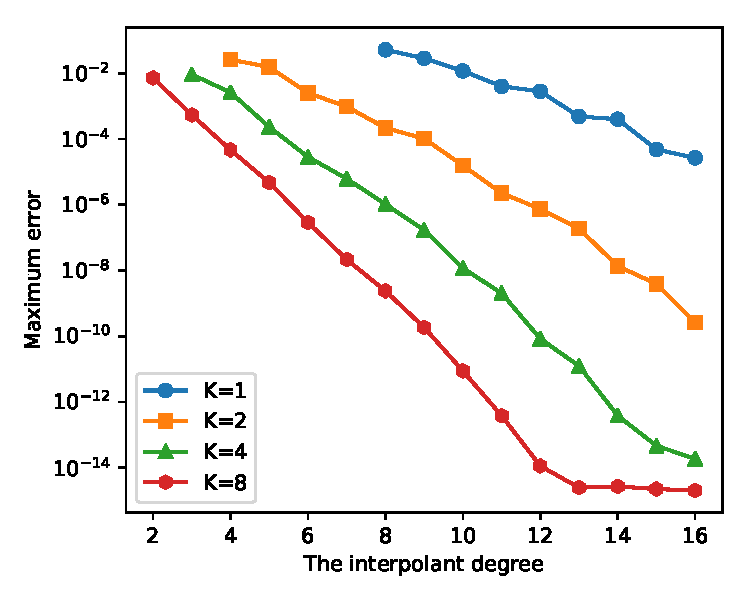
\includegraphics{tex/figures/interpolant_error}
	\fautor
	\label{fig:interpolant_error}
\end{figure}

\begin{figure}
	\centering
	\caption{The interpolation error measured on roots that were found after three Newton's iterations.}
	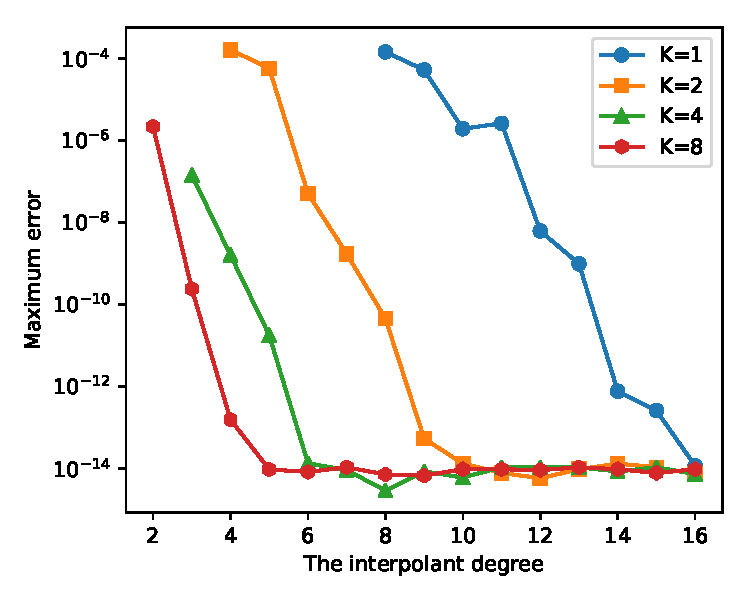
\includegraphics{tex/figures/interpolant_error_after_newton}
	\fautor
	\label{fig:interpolant_error_after_newton}
\end{figure}


\section{An Algorithm for MCER}\label{section:mcer}

\section{Implementation Details}\label{section:implementation}

\section{Numerical Experiments}\label{section:numerical}

\section*{References}
	%% New version of the num-names style
	\bibliographystyle{elsarticle-num}
	\bibliography{../references}
	
\end{document}

%%
%% End of file `elsarticle-template-1-num.tex'.